\chapter{Resumen y Conclusiones}
\label{chap:conclusions}
\thispagestyle{empt
%Write Conclusions, discussions, etc. here
%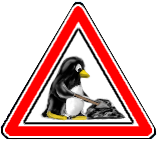
\includegraphics[width=0.1\linewidth]{./Figures/tux-development}

Hemos desarrollado un método para caracterizar la forma geométrica de choques de proa comparando dos parámetros adimensionales: la \textit{planitud} $\Pi$ del ápex del choque, y la \textit{alatud} $\Lambda$, o abertura de las alas. Ambos pueden ser medidos como los cocientes de longitudes que pueden ser medidas fácilmente. Desarrollamos un método (\S \ref{sec:projection}) para encontrar la forma aparente $(\Pi', \Lambda')$ de un choque abrillantado al limbo que es idealizado como cilíndricamente simétrico, en función del ángulo de inclinación $i$. Aplicamos este resultado a las cuádricas de revolución (capítulo \ref{chap:Modelo-generico}) y a la forma de los choques resultantes del modelo de capa delgada de interacción de dos vientos de \CRW{}, que están clasificados como wilkinoides, cantoides y ancantoides (capítulo \ref{chap:hipersonica}), y a observaciones en óptico de los choques de proa observados en la vecindad del Trapecio, en el centro de ONC (capítulo \ref{chap:proplyds}).

Aunque ya se han hecho análisis a las formas geométricas de los choques de proa (\citet{Robberto:2005}, ver figura \ref{fig:Robberto}), no se había utilizado antes el parámetro de la \textit{planitud} que siempre puede ser medido, a diferencia de la alatud, como ya ejemplificamos en el capítulo \ref{chap:proplyds}.

A pesar de que mucho del contenido de la \S \ref{sec:projection} ya había sido reportado en \citet{Wilkin-thesis} (apéndice B), las ecuaciones mostradas en esta sección fueron desarrolladas de manera independiente.

Se introdujo el diagrama $\Pi-\Lambda$ como una manera de caracterizar la forma de chques de proa. Las cuádricas de revolución sirven para caracterizar distintas regiones de este diagrama, y sirven como primera aproximación a la forma geométrica de otras superficies más complicadas.

En el modelo de capa delgada de \CRW{} (capítulo \ref{chap:hipersonica}), los escenarios que forman los choques cantoides y wilkinoides forman parte del trabajo de \CRW{}, siendo los choques ancantoides una extensión a este modelo. Por otro lado, el término \textit{wilkinoide} fue acuñado inicialmente por \citet{Cox:2012}, y a partir de ese nombre se acuñaron los términos \textit{cantoide} y \textit{ancantoide}.

Las mediciones del radio aparente en el ápex de los choques de proa cercanos al Trapecio en ONC concuerdan con las mediciones realizadas por \citet{Robberto:2005} (excepto por LV3). Además, comparando la forma aparente en un diagrama $(\Pi'-\frac{R'_0}{D'})$ de los choques con la forma aprente que predicen los modelos de capa delgada de \CRW{}. Encontramos los parámetros $(\beta, k, i)$ en los que coinciden los modelos con las observaciones. A partir de estos parámetros y utilizando las mediciones del radio del Frente de Ionización de cada proplyd medidos en \citet{HA:1998}, la tasa de pérdida de masa y la velocidad terminal de \thC{} de \citet{Gagne:2005}, dos modelos para estimar la densidad máxima del Frente de Ionización de los proplyds y números de Mach del flujo evaporado en el rango $[2, 3]$, encontramos que la dependencia con el número de Mach no es muy fuerte, que en el modelo A para estimar la densidad del IF del proplyd no existe correlación entre la presión encontrada con la distancia a \thC{}, mientras que en el modelo B sí existe. En trabajos posteriores se piensa analizar con el diagrama $\Pi-\Lambda$ a las clases de choque de proa mencionados en las \S \ref{sec:Luis-LL}, \ref{sec:runaway} y \ref{sec:AGBs}.